\chapter{Ausblick}

Sowohl durch den Industriepartner als auch durch das Team selbst kamen verschiedene Ideen für weitergehende Features auf. Aus Zeitgründen konnten leider nicht alle Ideen umgesetzt werden.

\section{'Workflow'}

Ein Wunsch der Industriepartner war es, den momentanen Arbeitsablauf abbilden zu können. Ein Beispiel ist, dass zuerst die 'unkritischen' Pakete auf den 'unkritischen' Systemen installiert werden müssen, bevor dort 'kritische' Pakete installiert werden können.

Dies wurde im 'Workflow'-Feature als Vorschlag präsentiert (Bild \ref{fig:ausblick:workflow}). Hier gibt es eine definierbare Reihenfolge von Arbeitsschritten, welche nacheinander durchgeführt werden müssen. Diese Arbeitsschritte könnten manuell festgelegt und bearbeitet sowie sortiert werden (Siehe Bild \ref{fig:ausblick:workflow_crud} für den Edit-Modus).

\begin{figure}[H]
	\centering
	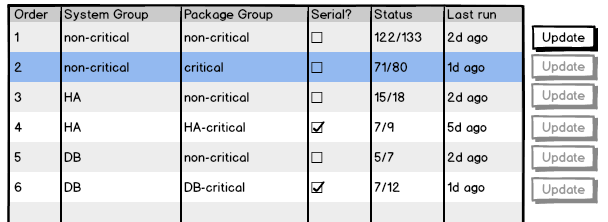
\includegraphics[width=0.75\linewidth]{files/mockups/workflow_smaller}
	\caption{Konzept Workflow-Feature}
	\label{fig:ausblick:workflow}
\end{figure}

\begin{figure}[H]
	\centering
	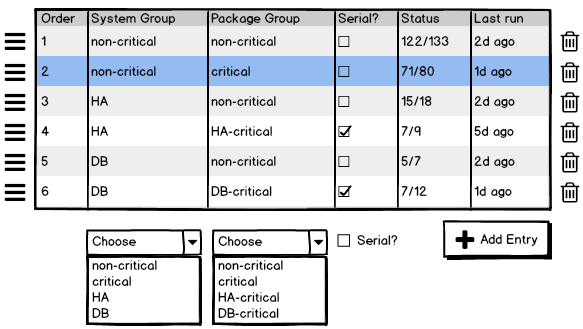
\includegraphics[width=0.75\linewidth]{files/mockups/workflow_CRUD_smaller}
	\caption{Konzept Workflow-Feature bearbeiten}
	\label{fig:ausblick:workflow_crud}
\end{figure}

\section{Dry-Run}

In \gls{apt} existiert das Feature 'dry-run', womit ein Updatevorgang simuliert\footnote{es werden keine Updates installiert, siehe auch \purl{http://linux.die.net/man/8/apt-get}} werden kann. Dies könnte auch als Feature im \gls{controlcenter} implementiert werden, indem vor dem Versenden eines Tasks zuerst eine Simulation durchgeführt werden könnte, um zu sehen, welche Pakete Abhängigkeiten nach sich ziehen oder fehlschlagen würden.

\section{Message-Queue}
\label{sec:ausblick:message_queue}

Mehrmals kam das Thema einer Message Queue auf. Die umgesetzt Lösung lässt das Control Center mit den Agenten einzeln kommunizieren, jeder Agent meldet sich direkt beim Control Center. Ein Nachteil davon ist, dass bei einem Absturz vom Control Center die Nachrichten zwar nicht verloren gehen, aber vom Agent erneut gesendet werden müssen. Bei einer längeren Unerreichbarkeit vom Control Center können sich so viele Nachrichten ansammeln, welche von den Agenten in regelmässigen Abständen wieder verschickt werden. Ist das Control Center wieder erreichbar, erhält es ein Mehrfaches an Nachrichten als normalerweise üblich. 

Mit einer Message Queue wäre dieses Problem weniger kritisch. Nachrichten werden zwischengespeichert, bis das Control Center wieder online ist.

Die Nachteile einer Message Queue sollten aber nicht unterschätzt werden. Einerseits wird der Single Point of Failure vom Control Center zur Message Queue verschoben und der Benutzer kann nicht arbeiten, wenn das Messaging-System ausfällt, andererseits bringt dieses Messaging-System eine neue Abhängigkeit mit sich.

\xxx[Benötigt offene Verbindung von A zu MQ...]

\section{Automatische Gruppen-Zuweisung}
\label{sec:ausblick:auto_group_assignment}

Ein optionaler Punkt aus der Aufgabenstellung (Kapitel \ref{sec:anforderung:aufgabenstellung}) waren Vorschläge der Applikation für System oder Pakate bezüglich der Gruppenzuteilung. Aufgrund von einfachen Regeln wie z.B. dem Namen oder einer IP-Range bei Systemen oder der 'Section'\footnote{Datenfeld bei apt-Paketen} bei Paketen könnten Vorschläge gemacht werden, zu welchen Gruppen etwas gehört.

In den Mockups wurde ein solches Feature bereits in groben Zügen angedacht (siehe Abbildung \ref{fig:ergebnis:group_systems_detail}). Pro System könnte die Auto-Zuweisung auch separat aktiviert und konfiguriert werden.

\begin{figure}
    \centering
    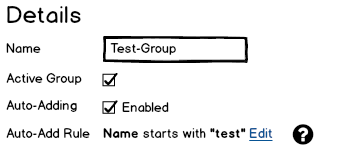
\includegraphics{files/mockups/group_systems_detail}
    \caption{Automatische Gruppenzuweisung für Systeme (Detail)}
    \label{fig:ergebnis:group_systems_detail}
\end{figure}

\section{Einfachere Registrierung}
\label{sec:ausblick:simple_registration}

Bei der aktuellen Lösung muss das Signierte Zertifikat beim Deployment vom Agenten mit ausgeliefert werden (siehe auch Kapitel \ref{sec:security}). Einfacher wäre es, wenn der Agent beim ersten Kontakt mit dem Control Center sich sein Zertifikat signieren lässt.

\xxx[ Separater API-Endpunkt für einfachere Registrierung, wie Puppet ]
\xxx[ korrekt? ]

\section{Geplante Tasks}
\label{sec:ausblick:scheduled_tasks}

Ein zu Beginn vorgesehenes aber aufgrund von anderen Prioritäten verworfenes Feature war die Möglichkeit, Tasks auf einen gewissen Zeitpunkt hin zu planen. Der Benutzer kann ein Datum und eine Uhrzeit eingeben, welche dann mit dem Task an den Agent übermittelt wird. Dieser plant die Ausführung selbst ein und meldet sich nach Abschluss des Tasks wieder beim Control Center.

Dies hätte auch die Möglichkeit ergeben, einen geplanten Task wieder abbrechen zu können, solange er noch nicht ausgeführt worden ist, womit die \gls{api} auf Agenten-Seite hätte erweitert werden müssen.

Ein Grund gegen dieses Feature war der Wunsch des Industriepartners, dass alle Tasks manuell durch einen Menschen ausgelöst werden müssen. Dies reduziert auch potentielle Probleme mit der Applikation, da Fehler zeitnah und nicht erst bei der Ausführung des Tasks auftauchen würden.

\section{Regelwerk}
\label{sec:ausblick:regelwerk}

Ein Feature, welches oft diskutiert aber schlussendlich nicht umgesetzt wurde, ist das Regelwerk. Dahinter steckt ein Mechanismus, welcher Abhängigkeiten innerhalb von verschiedenen System- und Paketgruppen generiert und kontrolliert. Ein Beispiel für eine solche Abhängigkeit ist etwa, dass nicht alle 'High-Availability'-Systeme auf einmal aktualisiert werden dürfen, da so möglicherweise kurze Ausfälle entstehen könnten. 

Dieses Feature wurde aber aufgrund von zu hoher Komplexität und fehlender Zeit verworfen. Ein Mockup ist in der Abbildung \ref{fig:ergebnis:rules} zu sehen.

\begin{figure}[H]
	\centering
	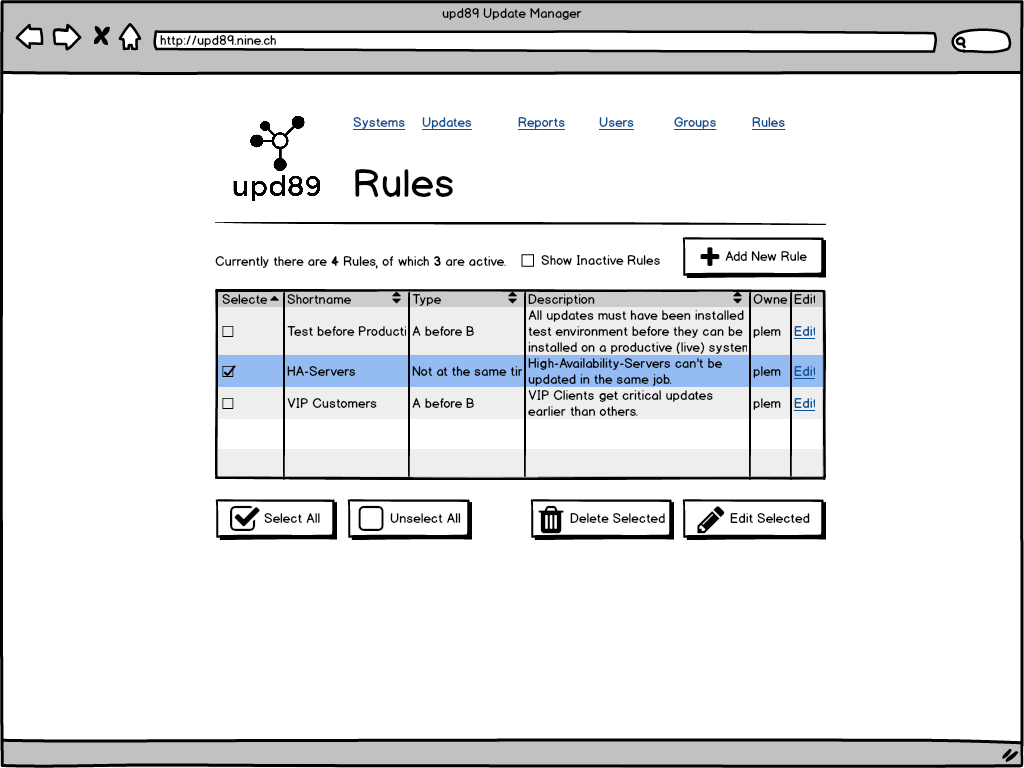
\includegraphics[width=\linewidth]{files/mockups/rules}
	\caption{Verworfenes Regelwerk-Feature}
	\label{fig:ergebnis:rules}
\end{figure}
